\documentclass[conference]{IEEEtran}
\IEEEoverridecommandlockouts
% The preceding line is only needed to identify funding in the first footnote. If that is unneeded, please comment it out.
\usepackage{cite}
\usepackage{amsmath,amssymb,amsfonts}
\usepackage{algorithmic}
\usepackage{algorithm}
\usepackage{graphicx}
\usepackage{textcomp}
\usepackage{xcolor}
\usepackage{enumitem}
\usepackage{booktabs}
\usepackage{tabularx}
\usepackage{pifont}
% \usepackage{titlesec}
\usepackage{balance}
\usepackage{tablefootnote}

\def\BibTeX{{\rm B\kern-.05em{\sc i\kern-.025em b}\kern-.08em
    T\kern-.1667em\lower.7ex\hbox{E}\kern-.125emX}}
\begin{document}

\title{Self-Evolving Beyond Human-Crafted Experience for EDA Scripting}

\author{Anonymous Authors}

% \author{
% \IEEEauthorblockN{Yang Liu$^{1,*,\dagger}$, Shengbo Tong$^{1,2,*}$, Xiyuan Chen$^{1,3}$, Shiwei Hou$^{1}$, Sen Yuan$^{1}$,}
% \IEEEauthorblockN{Hao Wang$^{1}$, Yanfeng Li$^{1,\dagger}$, Hongwen Li$^{1,\dagger}$, Yiming Zhu$^{1}$, Zhuolun He$^{2,\dagger}$}, Wenjian Yu$^{2,\dagger}$
% \IEEEauthorblockA{
% $^{1}$CXMT, $^{2}$Tsinghua University, $^{3}$USTC\\
% paul.liu@cxmt.com, tsb23@mails.tsinghua.edu.cn\\
% $^{*}$These authors contributed equally to this work.\\
% $\dagger$Corresponding authors.
% }
% }

\maketitle

\begin{abstract}
The growing complexity of electronic systems demands efficient design flows, yet EDA scripting remains a bottleneck: proprietary APIs are sparsely documented, and errors often appear as silent failures or cryptic exceptions. Hand-crafted knowledge helps but is difficult to maintain as toolchains evolve. We present \textbf{ZhuLong-SE (Self-Evolution)}, an execution-grounded LLM agent that learns reusable knowledge from prior task traces. Building on ZhuLong~\cite{liu2026zhulong}, it enhances the task-level harness with API retrieval, documentation responses, isolated sandbox execution, and static checking, then adds governed cross-task self-evolution.
% The checker raises no flags on the 158 benchmark ground-truth solutions, providing a sanity check on this reference-code set.
Beyond solving individual tasks, ZhuLong-SE distills past execution traces into a three-tier memory store governed by ground-truth anchoring, disconfirmation filtering, held-out rollback, and anti-leakage retrieval. On the 158-task EDA-Eval-PyAether benchmark, the full task-level harness, with self-evolution disabled, achieves 92.4\% pass@1 and outperforms ZhuLong on all five tested LLM backbones. On a harder instance-disjoint test set, self-evolution from the bare configuration surpasses a human-crafted-experience baseline by 2.5 percentage points (80.0\% vs.\ 77.5\% pass@1).
% Controlled ablations characterize the observed effects of key harness components and the write- and read-side mechanisms identifiable under their respective experimental settings. These results provide evidence that governed experience reuse can modestly surpass human-crafted experience in EDA scripting.
% 电子系统复杂性的日益增长要求高效的系统级设计流程，然而EDA工具的脚本编写仍然是一个关键瓶颈：专有API文档稀疏，错误仅表现为静默失败或晦涩的运行时异常，使得试错效率低下且难以扩展。手工领域知识虽有帮助，但无法跟上快速演进的工具链。我们提出了\textbf{ZhuLong-SE（Self-Evolution）}——一个能够从历史任务执行轨迹中学习的基于执行反馈的LLM智能体。ZhuLong-SE在ZhuLong~\cite{liu2026zhulong}任务级框架之上增强了API检索与文档响应、改进了隔离沙箱执行和静态检查，随后增加了受治理的跨任务自进化。检查器未标记158个基准ground-truth解的任何问题，对该参考代码集进行了健全性检查。
% 在解决单个任务之外，ZhuLong-SE将过往执行轨迹蒸馏到三层记忆存储中，由真值锚定、证伪过滤、留出回滚和反泄漏检索加以治理。在包含158个任务的EDA-Eval-PyAether基准上，禁用自进化的完整任务级框架达到92.4\%的pass@1，并在五个受测LLM基座上均优于ZhuLong。在更难的实例不相交测试集上，从Bare配置开始的自进化超越了人工经验基线2.5个百分点（80.0\%对比77.5\%的pass@1）。受控消融刻画了关键框架组件以及写侧和读侧机制在各自实验设置下可识别的作用。这些结果提供了证据表明，受治理的经验复用能够适度超越EDA脚本编写中的人工经验。
\end{abstract}

\begin{IEEEkeywords}
System-level design methodologies, design knowledge reuse, LLM agents, EDA scripting, continual learning, self-evolution, memory reliability, PyAether.
% 系统级设计方法论，设计知识复用，LLM智能体，EDA脚本编写，持续学习，自进化，记忆可靠性，PyAether
\end{IEEEkeywords}

\section{Introduction}
\label{sec:introduction}

EDA scripting is challenging because tool APIs are tool-specific, sparsely documented, and exposed through SWIG bindings whose type rules differ from native Python. ZhuLong~\cite{liu2026zhulong} is the first work that established an execution-grounded LLM agent for EDA scripting that combines API retrieval, documentation inspection, and sandbox execution via unified MCP tools, augmented by an offline API self-exploration mechanism that infers undocumented API behaviors through counterfactual experimentation. On the EDA-Eval-PyAether benchmark, the system achieved 78.5\% pass@1, substantially outperforming a pure LLM baseline of 23.6\%. However, a critical limitation remained: the agent solved each task independently and did not learn from past execution traces, so its performance on new tasks did not improve over time.
% EDA脚本编写面临挑战，因为工具API具有工具特异性、文档稀疏，且通过SWIG绑定暴露，其类型规则与原生Python不同。ZhuLong~\cite{liu2026zhulong}首次建立了一个基于执行反馈的EDA脚本LLM智能体，通过统一的MCP工具组合API检索、文档查阅和沙箱执行，并辅以离线API自探索机制，通过反事实实验推断未文档化的API行为。在EDA-Eval-PyAether基准上，该系统达到了78.5\%的pass@1，显著优于23.6\%的纯LLM基线。然而，一个关键局限仍然存在：该智能体独立解决每个任务，并未从过去的执行轨迹中学习，因此在新任务上的性能不会随历史经验积累而提升。

Building on this task-level substrate, we introduce \textbf{self-evolution}: an offline system that distills execution traces into reusable knowledge and re-injects it into future tasks, with reliability gates that prevent unverified experience from misleading the agent. To provide reliable signals for self-evolution, we introduce a precision-optimized static checker for deterministic API misuse. It raises no error flags on the 158 benchmark ground-truth solutions, a sanity check limited to this reference-code set. Applying self-evolution to EDA scripting introduces two challenges. First, feedback is very \textbf{sparse}: the agent receives only a binary pass/fail from the hidden verifier. This is different from methods like SkillOpt~\cite{yang2026skillopt}, which assume dense per-step rewards. Without careful verification, distilled experience can mislead. Second, instance-disjoint evaluation risks cross-split answer copying: a held-out task may copy a training sibling's verbatim solution rather than transferring the underlying method, a problem recently observed in EvolveMem~\cite{evolvemem2026}.
% 在这一任务级基础之上，我们引入\textbf{自进化}：一个离线系统将执行轨迹蒸馏为可复用知识并重新注入未来任务，通过可靠性门控防止未经验证的经验误导智能体。为给自进化提供可靠信号，我们引入了针对确定性API误用的精度优化静态检查器；在基准任务的ground-truth解上未观察到误报，此健全性检查仅限于该参考代码集。将自进化应用于EDA脚本编写带来了两个挑战。第一，反馈是\textbf{稀疏}的：智能体仅从隐藏验证器收到二元的通过/失败信号——与SkillOpt~\cite{yang2026skillopt}不同，后者假设密集的逐步奖励。缺乏审慎验证时，蒸馏经验可能误导。第二，实例不相交评估存在跨划分答案复制风险：留出任务可能直接复制训练集同类任务的逐字解决方案，而非迁移其方法，这一问题近期也在EvolveMem~\cite{evolvemem2026}中被观察到。

We present \textbf{ZhuLong-SE (Self-Evolution)}, which extends the ZhuLong task-level substrate with enhanced API retrieval and documentation responses, improved sandbox isolation, and precision-optimized static checking, and then adds a self-evolution layer with reliability gating. To handle sparse feedback, we introduce ground-truth anchoring, scope-boundary reflection, disconfirmation-based filtering, and a held-out validation loop that rejects degrading rounds. Beyond post-hoc evaluation gating, we design structural anti-leakage retrieval via names-only injection and deterministic docstring generalization to reduce the risk of cross-split answer copying. These mechanisms are designed to provide methodological signals without injecting full call sequences, while an evolution round is retained only when held-out validation does not degrade beyond the acceptance threshold. On the held-out test set, this design achieves a higher mean pass@1 than the human-crafted-experience baseline.
% 我们提出了\textbf{ZhuLong-SE（Self-Evolution）}，在ZhuLong任务级基础之上增强API检索与文档响应、改进沙箱隔离并加入精度优化静态检查，随后增加带可靠性门控的自进化层。为处理稀疏反馈，我们引入真值锚定、范围边界反思、基于证伪的过滤，以及拒绝退化轮次的留出验证循环。在事后评估门控之外，我们还通过仅名称注入和确定性文档字符串泛化设计了结构化反泄漏检索，以降低跨划分答案复制的风险。这些机制旨在提供方法论信号而不注入完整调用序列，同时仅在留出验证未超过退化阈值时保留进化轮次。在留出测试集上，该设计取得了高于人工经验基线的平均pass@1。

Our contributions are as follows.
% 我们的贡献如下。

\begin{itemize}[leftmargin=*]
\item \textbf{Self-evolution as a design methodology for EDA automation.} 
We establish self-evolution---distilling execution traces into reusable knowledge and re-injecting them into future tasks---as a systematic methodology for system-level EDA scripting. To make it deployable under EDA's sparse feedback and opaque commercial APIs, we introduce three governance rules: ground-truth anchoring, on-demand pitfall retrieval, and validation-gated rollback.
% 自进化作为EDA自动化的一种设计方法论。
% 我们将自进化——将执行轨迹蒸馏为可复用知识并重新注入到未来任务中——确立为一种系统级的EDA脚本编写方法论。为使其在EDA稀疏反馈和不透明商业API条件下可部署，我们引入了三条治理规则：真值锚定、按需陷阱检索、以及验证门控回滚。

\item \textbf{A rigorous evaluation protocol against cross-split leakage.} 
We expose cross-split answer copying as a threat to trustworthy self-evolution evaluation, and propose a retrieval-time defense (names-only injection + docstring generalization) that removes full call sequences and task-specific details while preserving methodological transfer---establishing a protocol for future work on self-evolving design agents.
% 一个对抗跨划分泄漏的严格评估协议。
% 我们揭示了跨划分答案复制对可信自进化评估构成的威胁，并提出了一种检索时防御机制（仅名称注入+文档字符串泛化），在保留方法论迁移信号的同时移除完整调用序列和任务特定细节——为未来自进化设计智能体的研究建立了一个评估协议。

\item \textbf{Counterintuitive design insights from controlled ablation.} 
Controlled ablations on the 158-task EDA benchmark yield three observations: ground-truth anchoring prevents 12 of 24 failed-task traces from producing falsely verified entries; pitfall pre-injection reduces validation pass@1 by 8.0\,pp in our ablation; and names-only retrieval improves over full-sequence injection by 4.7\,pp. On the 40-task held-out test set, self-evolution from the Bare configuration reaches 80.0\% mean pass@1, compared with 77.5\% for the human-crafted-experience baseline, grounding these observations for future system-level design automation.
% 来自控制变量消融实验的反直觉设计洞察。
% 在158任务EDA基准上的受控消融得到三项观察：真值锚定阻止24条失败任务轨迹中的12条产生错误验证条目；在当前消融中，陷阱预注入使验证pass@1下降8.0个百分点；仅名称检索相比完整序列注入提升4.7个百分点。在40任务留出测试集上，从Bare配置开始的自进化达到80.0\%平均pass@1，而人工经验基线为77.5\%，为未来系统级设计自动化提供了实证依据。
\end{itemize}

\section{Related Work}
\label{sec:related_work}

\subsection{LLM for EDA Scripting}
\label{sec:rw_eda}

LLMs for chip design have largely targeted RTL generation: ChipNeMo, RTLCoder, AutoChip, and CodeV-R1~\cite{liu2023chipnemo,liu2024rtlcoder,thakur2023autochip,zhu2026qimeng} domain-adapt or fine-tune models for Verilog, relying on human-constructed testbenches, which is orthogonal to operating an EDA tool's API surface. The procedural-scripting strand has grown quickly: ChatEDA, ChaTCL, EDA-Copilot, iScript, FluxEDA, JARVIS, and AutoEDA~\cite{wu2024chateda,rui2025chatcl,xiao2025eda,xu2026iscript,chen2026fluxeda,lu2025autoeda,zhang2025jarvis} span flow planning, Tcl/Q\&A assistance, multi-agent collaboration, single-turn generation, and execution infrastructure. Within this strand, ZhuLong~\cite{liu2026zhulong} is the direct precursor to our work: it combines API retrieval, documentation inspection, sandbox execution, and offline API self-exploration, but solves tasks independently without reusing execution traces across tasks. Another closely related system is OpenROAD Agent~\cite{wu2025openroad}, which adds execution-feedback self-correction on an open physical-design tool, but fine-tunes the model and does not externalize cross-task experience. Our scenario shares its generate-execute-revise shape yet keeps the model frozen and judges pass/fail by real sandbox execution with hidden tests---addressing cross-task reuse through self-evolution rather than fine-tuning. The Agentic EDA survey~\cite{zang2025dawn} situates this line at L3 autonomy. Two gaps recur for a frozen-agent, hidden-test setting: none externalizes cross-task experience into a reliable, leakage-controlled store, and none carries a domain-level static check beyond the tool's own schema---both of which our system addresses.
% 面向芯片设计的LLM主要面向RTL生成：ChipNeMo、RTLCoder、AutoChip和CodeV-R1~\cite{liu2023chipnemo,liu2024rtlcoder,thakur2023autochip,zhu2026qimeng}通过领域适配或微调模型生成Verilog，依赖人工构建的测试台，这与操作EDA工具API层面正交。流程脚本编写方向发展迅速：ChatEDA、ChaTCL、EDA-Copilot、iScript、FluxEDA、JARVIS和AutoEDA~\cite{wu2024chateda,rui2025chatcl,xiao2025eda,xu2026iscript,chen2026fluxeda,lu2025autoeda,zhang2025jarvis}涵盖流程规划、Tcl/问答辅助、多智能体协作、单轮生成和执行基础设施。在这一方向中，ZhuLong~\cite{liu2026zhulong}是本文最直接的前置工作：它结合API检索、文档查阅、沙箱执行和离线API自探索，但各任务独立求解，不复用跨任务执行轨迹。另一项密切相关的系统是OpenROAD Agent~\cite{wu2025openroad}，它在开源物理设计工具上增加执行反馈自修正能力，但会微调模型且未外部化跨任务经验。我们的场景与其共享生成-执行-修正形态，但保持模型冻结，并通过真实沙箱执行和隐藏测试判断通过/失败——通过自进化而非微调实现跨任务重用。Agentic EDA综述~\cite{zang2025dawn}将这一方向定位为L3自主级别。对于冻结智能体、隐藏测试的场景，仍有两个缺口：现有工作没有将跨任务经验外部化到可靠且受泄漏控制的存储中，也没有提供超越工具自身模式的领域级静态检查——本文系统同时解决这两个问题。

\subsection{Self-Evolving Agents with Governed Memory}
\label{sec:rw_self_evolving}

A broad family of works equips agents with reusable external memory: skill libraries, cross-task insight distillation, hierarchical memory, and cognitive architectures~\cite{wang2023voyager,zhao2024expel,packer2023memgpt,sumers2023cognitive}, with CodeAct~\cite{wang2024executable} unifying the action space as executable Python. The survey by Zhang et al.~\cite{zhang2024memory} provides a comprehensive taxonomy of memory mechanisms for LLM agents. These works, however, generally assume an open world or a train/test-disjoint split, which sidesteps the same-task regression signal that our fixed-set setting must surface. DemoEvolve~\cite{demoevolve2026} explicitly studies sparse terminal feedback in harness evolution, but addresses it through human demonstrations—whereas our setting assumes no such external guidance.
% 大量工作为智能体配备了可重用的外部记忆：技能库、跨任务洞察蒸馏、分层记忆和认知架构~\cite{wang2023voyager,zhao2024expel,packer2023memgpt,sumers2023cognitive}，其中CodeAct~\cite{wang2024executable}将动作空间统一为可执行的Python。Zhang等人的综述~\cite{zhang2024memory}为LLM智能体的记忆机制提供了全面的分类体系。然而，这些工作通常假设开放世界或训练/测试不相交的划分，这规避了我们的固定集合设定必须面对的同一任务回归信号问题。DemoEvolve~\cite{demoevolve2026}明确研究了框架进化中的稀疏终端反馈，但通过人类示范来解决——而我们的设定假设不存在此类外部指导。

Treating the skill store as an optimization target, SkillOpt~\cite{yang2026skillopt} edits a single skill document under a held-out gate and observes that ``plausible textual diagnoses can still hurt,'' echoing our concern that unverified experience can mislead. SkillOS~\cite{ouyang2026skillos} learns curation via RL with a four-dimensional judge, and Trace2Skill has been explored in two complementary forms: Ni et al.~\cite{ni2026trace2skill} propose a general framework that distills execution trajectories into reusable skills through parallel trajectory analysis and inductive pattern consolidation, using a verifier primarily for quality filtering of the extracted skills; Du and Pinckney~\cite{du2026trace2skill} present a test-time scaling framework for hardware agents where dense verifier feedback actively drives the oracle-mutator-selector evolution loop. These works optimize on disjoint splits with relatively dense signal, whereas our sparse-pass/fail, fixed-set setting makes which-experience-to-trust more pressing than how to edit a document.
% 将技能存储视为优化目标，SkillOpt~\cite{yang2026skillopt}在留出门控下编辑单个技能文档，并观察到“看似合理的文本诊断仍然可能造成损害”，这与我们对未验证经验可能误导的担忧一致。SkillOS~\cite{ouyang2026skillos}通过四维评判器的强化学习来学习策展，Trace2Skill已从两个互补方向进行探索：Ni等人~\cite{ni2026trace2skill}提出了一个通用框架，通过并行轨迹分析和归纳模式整合将执行轨迹蒸馏为可复用技能，其中验证器主要用于蒸馏后技能的质量过滤；Du和Pinckney~\cite{du2026trace2skill}提出了一个面向硬件智能体的测试时扩展框架，其中密集验证器反馈主动驱动"预言机-变异器-选择器"进化循环。这些工作在不相交划分上优化，且信号相对密集，而我们的稀疏通过/失败、固定集合设定使得“信任哪些经验”比“如何编辑文档”更为紧迫。

Verifier-guided evolution brings the reward signal closer to our hidden-test setting. ReVeal~\cite{jin2025reveal} self-generates test cases for dense rewards, but self-generated tests can be gamed and do not substitute for a hidden verifier. Du and Pinckney~\cite{du2026trace2skill} share our hidden-verifier, no-answer framing but run online per task with physical isolation and task-wise skills; their finding that cross-task transfer is unreliable for heterogeneous RTL cautions how far logical-error knowledge should travel—a concern we address through governed memory and anti-leakage retrieval. EvoAgentBench~\cite{gao2026evoagentbench}, the most comparable benchmark, formalizes this tension with an ability-supported yet instance-disjoint split, finding that an Anchor Skill oracle helps while no automatic method sustains the gain.
% 验证器引导的进化使奖励信号更接近我们的隐藏测试设定。ReVeal~\cite{jin2025reveal}自我生成测试用例以获得密集奖励，但自我生成的测试可能被操纵，不能替代隐藏验证器。Du和Pinckney~\cite{du2026trace2skill}与我们共享隐藏验证器、无答案的框架，但在每个任务上在线运行，具有物理隔离和任务级技能；他们发现跨任务迁移在异构RTL上不可靠，这警示了逻辑错误知识应传播多远——我们通过受治理记忆和反泄漏检索来应对这一问题。EvoAgentBench~\cite{gao2026evoagentbench}是最具可比性的基准测试，通过能力支撑但实例不相交的划分形式化了这种张力，发现Anchor Skill预言机有帮助，但没有任何自动方法能维持其收益。

Several works inform the governance machinery underlying our approach: MUSE-Autoskill~\cite{lin2026muse} on refinement and reflection, Externalization~\cite{zhou2026externalization} and Reflexion~\cite{shinn2023reflexion} on memory artifacts and same-task iteration, and Governing Evolving Memory~\cite{lam2026governing} on System-2 verification. LastingBench~\cite{fang2025lastingbench} proposes counterfactual rewriting to safeguard benchmarks against knowledge leakage, underscoring the importance of our anti-leakage retrieval design. The central lesson is that evolving memory requires an external gate grounded in ground truth to remain reliable. Our method addresses this challenge under sparse pass/fail supervision and strict anti-leakage constraints.
% 若干工作为我们方法背后的治理机制提供了参考：MUSE-Autoskill~\cite{lin2026muse}涉及精炼和反思，Externalization~\cite{zhou2026externalization}和Reflexion~\cite{shinn2023reflexion}涉及记忆制品和同任务迭代，Governing Evolving Memory~\cite{lam2026governing}涉及系统2验证。LastingBench~\cite{fang2025lastingbench}提出通过反事实重写来保护基准免受知识泄露，凸显了我们反泄漏检索设计的重要性。反复出现的教训是：进化的记忆需要一个外部的、真值锚定的门控来保持可信赖——这在稀疏通过/失败和反泄漏约束下，正是我们的方法所解决的问题。

\section{Method}
\label{sec:method}

\begin{figure*}[t]
\centering
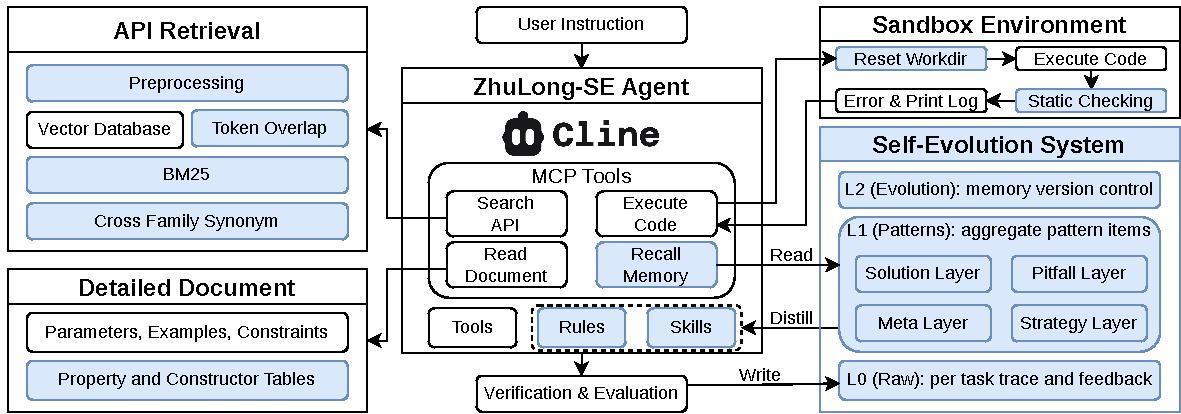
\includegraphics[width=1.0\textwidth]{figures/zhulong-se.pdf}
\caption{Architecture of ZhuLong-SE, adapted from the ZhuLong execution framework~\cite{liu2026zhulong}. Blue-highlighted blocks denote components added or enhanced in this work. Unhighlighted blocks show the shared execution workflow.}
\label{fig:architecture}
\end{figure*}

Building on the origin ZhuLong execution harness~\cite{liu2026zhulong}, ZhuLong-SE retains its retrieval--documentation--execution loop and introduces the blue-highlighted extensions in Figure~\ref{fig:architecture}: enhanced API retrieval and documentation, isolated parallel sandbox management, a precision-optimized static checker, human-crafted rules and skills, and an offline cross-task self-evolution system. We describe the task-level harness extensions in Sections~\ref{sec:method_retrieval}--\ref{sec:method_experience}, followed by self-evolution in Section~\ref{sec:selfev}.
% ZhuLong-SE建立在ZhuLong执行框架~\cite{liu2026zhulong}之上，保留其“检索—文档—执行”闭环，并引入图~\ref{fig:architecture}中以蓝色标出的扩展：增强的API检索与文档、隔离并行沙箱管理、精度优化静态检查器、人工编写的规则与技能，以及离线跨任务自进化系统。我们首先在第~\ref{sec:method_retrieval}至~\ref{sec:method_experience}节介绍任务级框架扩展，随后在第~\ref{sec:selfev}节介绍自进化系统。

\subsection{API Retrieval}
\label{sec:method_retrieval}

ZhuLong provides a single \texttt{search\_apis} MCP tool that uses semantic retrieval~\cite{liu2026zhulong}. ZhuLong-SE retains its embedding-based semantic path, adds a dedicated keyword-oriented tool (\texttt{search\_apis\_by\_keyword}), and supplements matches missed by the summary with a BM25 pass over the full description text. The keyword path targets queries that the semantic index handles poorly, such as abbreviations and camel-case fragments. The index tokenizes each API name by splitting on camel-case boundaries and stripping family prefixes. The query is bidirectionally expanded for abbreviations (e.g., CV$\leftrightarrow$CellView, crt$\leftrightarrow$create), enabling matches on abbreviated tokens inside API names. Depending on query type, a router expands abbreviations, returns direct-match hints for API-name fragments, or appends semantic results for natural-language queries. Finally, a cross-family synonym map links four functionally equivalent API families (db*, emy*, goa*, ae*), so a hit in one family surfaces equivalents in the others, addressing the failure mode where an agent recalls the correct operation but selects the wrong interface family.
% ZhuLong通过单一的\texttt{search\_apis}工具使用语义检索~\cite{liu2026zhulong}。ZhuLong-SE保留其基于嵌入的语义路径，新增专用的关键词工具\texttt{search\_apis\_by\_keyword}，并通过对完整描述文本的BM25检索补充摘要遗漏的匹配。关键词路径针对语义索引处理不佳的查询，如缩写和驼峰片段。索引通过驼峰边界拆分API名称并去除族前缀；查询则双向扩展缩写（例如CV$\leftrightarrow$CellView，crt$\leftrightarrow$create），从而匹配API名称中的缩写词元。路由器根据查询类型扩展缩写、为API名称片段返回直接匹配提示，或为自然语言查询追加语义检索结果。最后，一个跨族同义词映射连接四个功能等价的API族（db*、emy*、goa*、ae*），使命中一族时同时呈现其他族的等价项，解决智能体记得正确操作但选错接口族的问题。

\subsection{Documentation Enrichment}
\label{sec:method_doc}

ZhuLong's \texttt{get\_api\_details} returns parameter types, return values, examples, and inferred constraints~\cite{liu2026zhulong}, but its per-API pages do not expose class instance properties. ZhuLong-SE therefore parses the raw documentation into a property table and appends it to each detailed response, so a queried class exposes its instance attributes alongside its methods. Constructor notes also disambiguate ambiguous calls: for example, \texttt{emyPointArray} accepts a plain list of points, a fact the per-signature page does not state.
% ZhuLong的\texttt{get\_api\_details}返回参数类型、返回值、示例和推断出的约束~\cite{liu2026zhulong}，但其逐API页面不公开类的实例属性。ZhuLong-SE因此将原始文档解析为属性表并附加到每个详细响应，使查询到的类在方法之外也暴露实例属性。构造函数注释还消除了模糊调用的歧义：例如，\texttt{emyPointArray}接受普通点列表，而逐签名页面并未说明这一事实。

\subsection{Sandbox Execution}
\label{sec:method_sandbox}

We run multiple isolated sandbox endpoints, each with an independent working directory, and dispatch requests through a queue pool. A routine clears working directories before each run and resets library files to minimal content, so prior runs do not bias subsequent ones. This isolation ensures that execution feedback reflects the current code under test, not residual state from earlier tasks. The queue pool enables concurrent evaluation without changing ZhuLong's per-task interaction protocol~\cite{liu2026zhulong}.
% 我们运行多个隔离的沙箱端点，每个端点拥有独立工作目录，并通过队列池分派请求。一个例行程序在每次运行前清空工作目录并将库文件重置为最小内容，使先前运行不会影响后续运行。这种隔离确保执行反馈反映当前被测试代码，而非先前任务的残留状态。队列池在不改变ZhuLong逐任务交互协议~\cite{liu2026zhulong}的前提下支持并发评估。

\subsection{Static Checking}
\label{sec:method_checker}

Because PyAether's SWIG bindings expose all symbols at import time regardless of whether the underlying function exists at runtime, an agent may call a fabricated API or pass a native Python value where a SWIG-wrapped type is required without triggering any runtime error during self-test—yet the submission fails the hidden test that exercises that path. To catch such failures before submission, we introduce a static checker that runs after the agent's self-test and before final submission.
% 由于PyAether的SWIG绑定在导入时暴露所有符号，而不管底层函数在运行时是否存在，智能体可能调用捏造的API或将原生Python值传递给需要SWIG封装类型的位置，而不会在自测期间触发任何运行时错误——但提交会在执行该路径的隐藏测试中失败。为了在提交前捕获此类失败，我们引入了一个静态检查器，在智能体自测之后、最终提交之前运行。

The checker parses submitted code into an abstract syntax tree, extracts API calls, and checks four documented misuse patterns: (i) fabricated APIs, (ii) incorrect keyword arguments, (iii) native Python values passed where explicit SWIG-wrapped construction is required, and (iv) silently swallowed exceptions. Actionable findings are returned to the agent for repair before final submission. The rules are derived from the API documentation and refined on real submissions. As a reference-code sanity check, the checker raises no flags on any of the 158 ground-truth solutions. This result is limited to that set and is not a general zero-false-positive guarantee.
% 检查器将提交的代码解析为抽象语法树，提取API调用，并检查四类已记录的误用模式：（i）捏造的API，（ii）错误的关键字参数，（iii）传递给需要显式SWIG封装构造的参数的原生Python值，以及（iv）被吞没的异常。可操作的发现被返回给智能体，以便在最终提交前修复。规则来源于API文档，并在真实提交上进行精炼。作为参考代码的健全性检查，检查器未对158个ground-truth解中任何一个标记问题；此结果仅限于该集合，并非一般性的零误报保证。


\subsection{Human-Crafted Experience}
\label{sec:method_experience}

ZhuLong-SE additionally injects four skills and one rule file authored from PyAether development experience rather than specific benchmark solutions. The skills cover API search, command-family selection, interpretation of silent or ambiguous sandbox feedback, and explicit SWIG type construction. The rule file requires API-detail checks before use, post-creation verification, and bounded search, providing a stable prior that complements knowledge learned from the execution traces.
% ZhuLong-SE还注入四条技能和一条规则文件，这些内容来源于PyAether开发经验而非基准任务的解答。技能涵盖API搜索、命令族选择、静默或模糊沙箱反馈的解读，以及显式SWIG类型构造。规则文件要求在使用前进行API详情检查、创建后验证和有限搜索，提供了一个稳定的先验知识，与执行轨迹学到的知识形成互补。

\section{Self-Evolution}
\label{sec:selfev}

Unlike ZhuLong's offline API self-exploration, which augments per-API documentation through counterfactual sandboxing~\cite{liu2026zhulong}, ZhuLong-SE adds a cross-task offline self-evolution system (the blue-highlighted block at right in Figure~\ref{fig:architecture}). It distills task execution traces into reusable knowledge and re-injects it into later tasks. Knowledge is organized in three tiers, following the episodic-semantic-procedural memory distinction~\cite{sumers2023cognitive}: \emph{L0} holds raw traces, \emph{L1} stores aggregated patterns, and \emph{L2} archives distilled skill versions. Within L1, patterns are partitioned into four layers: \emph{solution} (verified API routes), \emph{pitfall} (negative warnings), \emph{meta} (effective query patterns), and \emph{strategy} (decision records). The write side runs offline after each training batch, and the read side injects knowledge at task formatting and on demand when the agent hits an error. The write, promotion, and round-acceptance stages apply reliability gates, as unvalidated experience can mislead~\cite{zhao2024expel,yang2026skillopt}. Distillation and state updates run offline. During inference, the accepted memory is queried locally, without additional evolution or distillation.
% ZhuLong的离线API自探索通过反事实沙箱实验增强逐API文档~\cite{liu2026zhulong}；与之不同，ZhuLong-SE增加了跨任务离线自进化系统（图~\ref{fig:architecture}右侧蓝色模块）。该系统将任务执行轨迹蒸馏为可复用知识，并将其重新注入后续任务。知识按照情节—语义—程序性记忆的区分组织为三个层级~\cite{sumers2023cognitive}：\emph{L0}保存原始轨迹，\emph{L1}存储聚合模式，\emph{L2}归档蒸馏出的技能版本。在L1内部，模式分为四层：\emph{solution}（已验证API路径）、\emph{pitfall}（负面警告）、\emph{meta}（有效查询模式）和\emph{strategy}（决策记录）。写入侧在每个训练批次后离线运行；读取侧在任务格式化时以及智能体遇到错误时按需注入知识。写入、晋升和轮次接受阶段应用可靠性门控，因为未经验证的经验可能造成误导~\cite{zhao2024expel,yang2026skillopt}。蒸馏和状态更新离线执行；推理期间仅在本地查询已接受的记忆，不进行额外进化或蒸馏。

\subsection{Distillation and Reflection}
\label{sec:se_distill}

The write side routes each task to the appropriate reflection path. We override the agent's self-reported success with the evaluator's binary verdict before any reflection begins, following Reflexion's observation that reliable feedback is necessary for reflection to help rather than harm~\cite{shinn2023reflexion}. Tasks that still error on their final attempt take the \emph{error path}; tasks whose self-test passed but the evaluator failed take the \emph{contradiction path} instead. This distinction is critical because a self-test-passed task's error log contains only stale errors; mining pitfalls from these would record already-solved bugs rather than genuine gaps in the agent's knowledge. Each L1 entry carries a reliability tier: \emph{verified}, \emph{unverified}, or \emph{pitfall}.
% 写入侧将每个任务路由到相应的反思路径。我们在任何反思开始之前用评估器的二元判定覆盖智能体自报告的成功，遵循Reflexion的观察——可靠的反馈是反思起作用而非造成伤害的必要条件~\cite{shinn2023reflexion}。在最终尝试中仍然出错的任务走\emph{错误路径}；自测通过但评估器失败的任务则走\emph{矛盾路径}。这种区分至关重要，因为自测通过的任务的错误日志只包含过时错误；从中挖掘陷阱会记录已解决的错误而非智能体知识中的真正空白。每个L1条目带有一个可靠性等级：\emph{verified}、\emph{unverified}或\emph{pitfall}。

\subsection{Knowledge Lifecycle with Reliability Gating}
\label{sec:se_govern}

Extracted L1 patterns undergo aggregation, gating, aging, and promotion to rules and skills. A verified entry is disconfirmed only when a failed task is an API misuse precisely attributed to that entry; at a count of two or more, the entry is filtered out. Unverified traces cannot downgrade verified entries, and entries not re-confirmed for five rounds drop to unverified. Promotion is guarded by a four-dimensional judge (abstraction, reusability, actionability, faithfulness) following SkillOS~\cite{ouyang2026skillos}, and a MUSE-style create-evaluate-refine loop~\cite{lin2026muse} for low-scoring candidates. We add a zero-exception generality gate that rejects rules whose always/never statements do not hold across the entire API surface, ensuring that distilled rules remain broadly applicable rather than overfitting to specific task patterns.
% 提取的L1模式经历聚合、门控、老化以及提升为规则和技能。一个已验证条目仅当一个失败任务是被精确定位到该条目的API误用时才被证伪；达到两个或以上时，该条目被过滤掉。未经验证的轨迹不能降级已验证条目，连续五轮未重新确认的已验证条目降级为未验证。提升由两个质量机制把关：遵循SkillOS~\cite{ouyang2026skillos}的四维评判器（抽象性、可重用性、可操作性、忠实性），以及一个针对低分候选的MUSE风格创建-评估-精炼循环~\cite{lin2026muse}。我们增加了一个零异常泛化门控，拒绝任何在全API表面上不成立的always/never语句的规则——确保蒸馏出的规则保持广泛适用性而非过拟合特定任务模式。

\subsection{Anti-Leakage Retrieval}
\label{sec:se_read}

Under an instance-disjoint split, naive retrieval risks cross-split answer copying. We prevent this through three mechanisms. \textbf{Names-only pre-injection} reduces a solution entry to API names only, dropping call order and parameters. \textbf{Deterministic docstring generalization} strips task-identifying specifics from both distillation and query sides. \textbf{Problem-side embedding} matches on problem similarity while returning solution metadata only at read time. Pitfalls are not pre-injected; they enter through on-demand runtime queries keyed to the agent's actual error.
% 在实例不相交划分下，朴素的检索存在跨划分答案复制的风险。我们通过三个机制来防止这一问题。\textbf{仅名称预注入}将solution条目缩减为仅API名称，丢弃调用顺序和参数。\textbf{确定性文档字符串泛化}从蒸馏侧和查询侧同时移除任务标识性细节。\textbf{问题侧嵌入}在问题相似性上进行匹配，同时仅在读取时返回解决方案元数据。Pitfalls不预注入；它们通过以智能体实际错误为键的按需运行时查询进入。

\subsection{Held-Out Gated Evolution}
\label{sec:se_loop}

After each training round, the agent generates on validation tasks (which never carry distillation). The round's full evolved state is accepted only if the validation pass rate does not regress by more than 5~pp against the previous round. Otherwise, it is rolled back. This extends SkillOpt's held-out criterion~\cite{yang2026skillopt} from a single document to the entire evolved state.
% 每轮训练后，智能体在验证任务上生成（验证任务从不参与蒸馏）。该轮完整进化状态仅在验证通过率相比上一轮被接受的轮次不倒退超过5\%时才被接受；否则从快照回滚。这将SkillOpt的留出准则~\cite{yang2026skillopt}从单个文档扩展到整个进化状态。

\section{Experiments}
\label{sec:experiments}

We evaluate ZhuLong-SE on EDA-Eval-PyAether, the 158-task real-world PyAether scripting benchmark introduced by ZhuLong~\cite{liu2026zhulong}\footnote{We obtained the benchmark by contacting its authors.}. Each task is a natural-language docstring plus a function signature, and a submission passes only if real sandbox execution satisfies a hidden test (the black-box verifier). The primary model is DeepSeek-V4-Pro-Preview. The human-crafted experience consists of four skills and one rule authored by a senior EDA engineer with extensive experience in PyAether development.
% 我们在EDA-Eval-PyAether上评估ZhuLong-SE；该基准由ZhuLong~\cite{liu2026zhulong}提出，包含158个真实PyAether脚本任务。每个任务由自然语言docstring和函数签名组成，提交仅在真实沙箱执行满足隐藏测试（黑盒验证器）时通过。主要模型为DeepSeek-V4-Pro-Preview。人工编写经验由四条技能和一条规则组成，作者是一位具有丰富PyAether开发经验的高级EDA工程师。

The experiments have two parts. First, on all 158 tasks, we ask whether the enhanced ZhuLong-SE harness outperforms the original ZhuLong across matched LLM backbones and which measured harness components contribute to the gain. Second, after removing human-crafted experience, we ask whether governed self-evolution can match or surpass the human-crafted-experience baseline.
% 实验分为两部分。第一部分在全部158个任务上考察增强后的ZhuLong-SE任务级框架是否在匹配的LLM基座上优于原始ZhuLong，以及哪些可测量的框架组件对增益作出贡献。第二部分移除人工编写经验，考察受治理的自进化能否匹配或超过人工经验基线。

\subsection{Harness Evaluation}
\label{sec:exp_retrieval}

We first evaluate the enhanced task-level harness, with self-evolution disabled throughout this subsection. The complete ZhuLong-SE configuration enables all harness enhancements described in Section~\ref{sec:method}, including full retrieval, documentation enrichment, sandbox isolation, the static checker, and human-crafted experience. We first compare this configuration with the published ZhuLong baseline and then decompose the measured components under the primary backbone. No self-evolved knowledge is injected into any result reported in this subsection. For each comparison, the backbone version and settings other than the harness components under study are aligned with ZhuLong~\cite{liu2026zhulong}. Table~\ref{tab:cross_method} uses the reported ZhuLong results where available.
% 我们首先评估增强后的任务级执行框架，本小节始终禁用自进化。完整的ZhuLong-SE配置启用了第~\ref{sec:method}节所述的全部框架增强，包括完整检索、文档增强、沙箱隔离、静态检查器和人工编写经验。我们首先将该配置与已发表的ZhuLong基线进行比较，随后在主要基座模型上分解可独立测量的组件。本小节报告的所有结果均未注入自进化知识。对于每个基座匹配的比较，除被研究的框架组件外，其余设置均与ZhuLong~\cite{liu2026zhulong}所报告的设置对齐；表~\ref{tab:cross_method}中的ZhuLong结果直接取自该论文，而非由本文重新运行。

Table~\ref{tab:cross_method} compares ZhuLong-SE with ZhuLong on the same backbone versions. Across all the five comparisons, ZhuLong-SE improves by 11.4~pp on DeepSeek-V4-Pro-Preview, 16.4~pp on GLM-5.2, 5.7~pp on Kimi-K2.6, 6.9~pp on DeepSeek-V4-Flash-Preview, and 15.8~pp on Doubao-Seed-2.0-pro. Because self-evolution is disabled, these gains reflect the combined task-level enhancements in Section~\ref{sec:method}. The comparisons indicate transfer across the tested model families, although absolute performance still depends on backbone capability.
% 表~\ref{tab:cross_method}在相同基座版本上比较ZhuLong-SE与ZhuLong。在五组对齐比较中，ZhuLong-SE在DeepSeek-V4-Pro-Preview上提升了11.4个百分点，GLM-5.2上提升16.4个百分点，Kimi-K2.6上提升5.7个百分点，DeepSeek-V4-Flash-Preview上提升6.9个百分点，Doubao-Seed-2.0-pro上提升15.8个百分点。由于自进化被禁用，这些提升反映了第~\ref{sec:method}节所述的全部任务级增强。这些比较表明跨模型族的迁移性，尽管绝对性能仍取决于基座能力。

\begin{table}[ht]
\caption{Harness-only Pass@1 comparison with ZhuLong on aligned backbone versions (158 tasks, one ZhuLong-SE run per model, no self-evolution). }
\label{tab:cross_method}
\setlength{\tabcolsep}{2pt}
\centering
\small
\begin{tabular}{lccr}
\toprule
Model & ZhuLong & ZhuLong-SE & $\Delta$ \\
\midrule
DeepSeek-V4-Pro-Preview   & 81.0\% & 92.4\% & +11.4~pp \\
GLM-5.2                   & 74.7\% & 91.1\% & +16.4~pp \\
Kimi-K2.6                 & 83.5\% & 89.2\% & +5.7~pp \\
DeepSeek-V4-Flash-Preview & 78.5\% & 85.4\% & +6.9~pp \\
Doubao-Seed-2.0-pro       & 55.7\% & 71.5\% & +15.8~pp \\
\bottomrule
\end{tabular}
\end{table}

Each harness configuration is evaluated once because a full 158-task run is costly, and the broad task coverage reduces sensitivity to any single task outcome. Repeated runs are reserved for the smaller validation and challenge-test evaluations.
% 每个框架配置仅评估一次，因为完整的158个任务运行成本高昂。广泛的任务覆盖降低了对单个任务结果的敏感度；因此重复运行仅保留给规模较小的验证集和挑战测试评估。

% \begin{table}[ht]
% \caption{Cross-model generalization: same Full-retrieval, Human-crafted configuration across five LLMs (single run, 158 tasks). Tokens are summed over all tasks.}
% \label{tab:cross_model}
% \centering
% \small
% \begin{tabular}{lcrr}
% \toprule
% Model & Pass@1 & Time & Token \\
% \midrule
% DeepSeek-V4-Pro-Preview   & 92.4\% & 22.5\,h & 114.8\,M \\
% GLM-5.2                   & 91.1\% & 28.0\,h & 128.0\,M \\
% Kimi-K2.6                 & 89.2\% & 22.7\,h & 126.2\,M \\
% DeepSeek-V4-Flash-Preview & 85.4\% & 11.1\,h & 134.0\,M \\
% Doubao-Seed-2.0-pro       & 71.5\% & 7.5\,h  & 28.3\,M \\
% \bottomrule
% \end{tabular}
% \end{table}

We next perform an ablation study on ZhuLong-SE. Because ZhuLong-SE is inherited from ZhuLong, we use progressive rather than leave-one-out ablation to attribute that advantage to the newly added components. Checker \emph{ON} enables the static checker, whereas \emph{OFF} bypasses it. \emph{Semantic-Only} retains \texttt{search\_apis} but disables the keyword tool and BM25 supplement, whereas \emph{Full} enables both tools. \emph{Bare} uses no human-crafted knowledge, whereas \emph{Human} adds four skills and one rule derived from human PyAether development experience rather than the benchmark tasks. DeepSeek-V4-Pro-Preview serves as the fixed inference backbone. Table~\ref{tab:ablation} shows that successive additions raise Pass@1 from 81.0\% to 87.3\% with the checker (+6.3~pp), to 88.6\% with Full retrieval (+1.3~pp), and to 92.4\% with Human experience (+3.8~pp). Each component therefore contributes, with the checker providing the largest stepwise gain. Documentation enrichment and sandbox isolation remain fixed and are evaluated only in the overall harness comparison.
% 由于ZhuLong-SE继承自ZhuLong，我们采用递进式而非逐项移除消融，以归因这一优势来自哪些新增组件。检索层包含两个级别：\emph{Full}（第~\ref{sec:method_retrieval}节）和\emph{Semantic-Only}，后者保留语义\texttt{search\_apis}路径，但禁用专用关键词工具和BM25补充。经验层也包含两个级别：\emph{Bare}不使用人工编写的技能或规则，\emph{Human}则包含四条人工技能和一条规则。这些资产来自PyAether平台开发期间积累的领域知识，并非通过检查或拟合158个基准任务得到，因此不构成测试集泄露。以关闭检查器的Bare、Semantic-Only配置为起点，后续各行依次加入检查器、Full检索和Human经验。
% 依次加入检查器、Full检索和Human经验后，Pass@1从81.0\%提高到87.3\%（+6.3个百分点）、88.6\%（+1.3个百分点）和92.4\%（+3.8个百分点）。各组件均有贡献，其中检查器的单步增益最大。文档增强与沙箱隔离保持固定，仅在整体框架比较中评估。

\begin{table}[ht]
\caption{Progressive harness ablation on the 158-task benchmark (single run, DeepSeek-V4-Pro-Preview).}
\label{tab:ablation}
\centering
\small
\begin{tabular}{lccr}
\toprule
Experience & Retrieval & Checker & Pass@1 \\
\midrule
Bare  & Semantic-Only & OFF & 81.0\% \\
Bare  & Semantic-Only & ON & 87.3\% \\
Bare  & Full          & ON & 88.6\% \\
% Human & Semantic-Only & ON & 89.9\% \\
Human & Full          & ON & 92.4\% \\
\bottomrule
\end{tabular}
\end{table}

% \begin{table}[ht]
% \caption{Retrieval--experience decomposition on the 158-task benchmark (single run, DeepSeek-V4-Pro-Preview). Time is wall-clock per run, and tokens are summed over all tasks.}
% \label{tab:retrieval_ablation}
% \centering
% \small
% \begin{tabular}{lccrr}
% \toprule
% Experience & Retrieval & Pass@1 & Time & Token \\
% \midrule
% Bare  & Semantic-Only & 87.3\% & 15.0\,h & 83.1\,M \\
% Bare  & Full          & 88.6\% & 15.8\,h & 75.3\,M \\
% Human & Semantic-Only & 89.9\% & 17.0\,h & 122.9\,M \\
% Human & Full          & 92.4\% & 22.5\,h & 114.8\,M \\
% \bottomrule
% \end{tabular}
% \end{table}

Task~132 illustrates why the keyword path complements semantic retrieval. The task connects two orthogonal routing paths by placing a via at their intersection and requires constructing several SWIG-wrapped types. With Semantic-Only retrieval, the agent issued natural-language queries but did not retrieve the required type definitions, eventually passing a native tuple where a wrapped object was required. With Full retrieval, the agent queried \texttt{ViaDef}, \texttt{emyPoint}, and \texttt{emyString} through the keyword path, retrieved their construction signatures, and completed the task successfully. This case reflects the intended role of camel-case splitting and exact-fragment matching: they make abbreviation-dense API and type names directly addressable when natural-language similarity is insufficient.
% Task~132说明了关键词路径为何能够补充语义检索。该任务需要在两条正交布线路径的交点放置过孔，并构造多个SWIG封装类型。在Semantic-Only检索下，智能体发出自然语言查询，但未检索到所需的类型定义，最终在需要封装对象的位置传入了原生tuple。在Full检索下，智能体通过关键词路径查询\texttt{ViaDef}、\texttt{emyPoint}和\texttt{emyString}，获得其构造签名并成功完成任务。该案例体现了驼峰拆分和精确片段匹配的预期作用：当自然语言相似度不足时，它们使缩写密集的API与类型名称可以被直接检索。

Finally, we characterize the residual failures of the enhanced harness. Figure~\ref{fig:failure_types} aggregates the 111 failed tasks across the five ZhuLong-SE backbone runs in Table~\ref{tab:cross_method}. \texttt{AssertionError} accounts for 54.1\% of these failures: the generated program reaches the hidden verifier without an uncaught API or type error, but its result violates a tested property. Such semantic or result-level errors lie outside the static checker's declared scope, which targets deterministic API misuse rather than hidden functional correctness. This analysis therefore characterizes the remaining failure frontier rather than directly measuring checker recall. Since the task-level harness still solves each task independently, these residual errors motivate the next subsection's evaluation of whether validated knowledge distilled from prior traces can improve later tasks.
% 最后，我们分析增强框架的剩余失败。图~\ref{fig:failure_types}汇总了表~\ref{tab:cross_method}中ZhuLong-SE在五个基座模型上的111个失败任务。其中，\texttt{AssertionError}占54.1\%：生成程序在没有未捕获API或类型错误的情况下到达隐藏验证器，但其结果违反了被测试的属性。这类语义或结果层面的错误超出了静态检查器的既定范围；检查器针对的是确定性API误用，而非隐藏的功能正确性。因此，该分析刻画的是剩余失败边界，而不是对检查器召回率的直接测量。由于任务级框架仍独立解决每个任务，这些剩余错误进一步引出下一小节：由先前轨迹蒸馏并经过验证的知识能否改善后续任务。

\begin{figure}[ht]
\centering
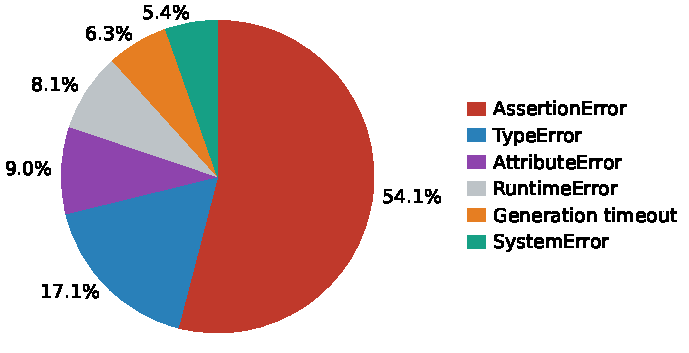
\includegraphics[width=\columnwidth]{figures/failure_type_distribution.pdf}
\caption{Residual failure types of ZhuLong-SE across five LLM backbones on the 158-task benchmark (111 failures aggregated).}
\label{fig:failure_types}
\end{figure}

\subsection{Self-Evolution}
\label{sec:exp_selfev}

To evaluate self-evolution without ceiling effects—the Bare agent already passes 87\% of the 158 tasks—and to support held-out gating, we adopt an instance-disjoint \emph{challenge split} (train~98 / val~20 / test~40), in the spirit of EvoAgentBench's ability-supported yet instance-disjoint split~\cite{gao2026evoagentbench}. The split is stratified so that the test set concentrates more discriminative tasks, identified by testbench code length and the number of unique APIs used. Because the validation and test sets are small, every self-evolution evaluation is the mean of \textbf{five} independent runs with its standard deviation.
% 为在没有天花板效应的情况下评估自进化——Bare智能体已通过158个任务中87\%——并支持留出门控，我们采用实例不相交的\emph{挑战划分}（训练98/验证20/测试40），遵循EvoAgentBench的能力支撑但实例不相交划分的精神~\cite{gao2026evoagentbench}。该划分经过分层，使测试集集中于更具区分度的任务——以测试台代码长度和使用的唯一API数量为标识。由于验证集和测试集较小，每个自进化评估均为\textbf{五次}独立运行的平均值及其标准差。

Table~\ref{tab:sevolution} reports test Pass@1 across rounds, against the Bare baseline (no evolved knowledge) and the Human baseline. Self-evolution clears the Bare baseline by +14.0~pp (66.0\%$\to$80.0\%) and surpasses the Human baseline (80.0\% vs.\ 77.5\%) at Round~2, after which Round~3 regresses to 75.5\%. The validation trend is consistent: validation peaks at Round~2 (88.0\%) and drops at Round~3 (80.0\%), so the gate accepts Rounds~1 and~2 but rejects Round~3, rolling back its 52 new entries and freezing the knowledge base at Round~2 (334 entries, 20 skills). Crucially, the test trend agrees with validation—Round~3 regresses on both (75.5\% vs.\ 80.0\%)—confirming the gate's rejection reflects genuine overfitting, not a validation-specific artifact. Round~2 also has the smallest observed run-to-run spread ($\pm$3.1), below the Human baseline's $\pm$5.3.
% 表~\ref{tab:sevolution}报告了各轮次测试Pass@1，对比Bare基线（无进化知识）和Human基线。自进化以+14.0个百分点（66.0\%$\to$80.0\%）超越Bare基线，并在第2轮超越Human基线（80.0\%对比77.5\%），之后第3轮退步至75.5\%。验证趋势一致：验证集在第2轮达到峰值（88.0\%），在第3轮下降（80.0\%），因此门控接受第1轮和第2轮但拒绝第3轮，回滚其52条新条目并将知识库冻结在第2轮（334条条目，20条技能）。关键的是，测试趋势与验证一致——第3轮在两者上均退步（75.5\%对比80.0\%）——确认门控的拒绝反映的是真正的过拟合而非验证集特有的假象。第2轮还具有观测到的最小跨运行波动（$\pm$3.1），低于Human基线的$\pm$5.3。

\begin{table}[ht]
\caption{Self-evolution on the challenge test set (40 tasks, 5 runs each, DeepSeek-V4-Pro-Preview). ``Patterns'' is the L1 entry count, ``skills'' are auto-distilled. The held-out gate accepted Rounds~1 and~2, and rejected Round~3.}
\label{tab:sevolution}
\setlength{\tabcolsep}{2.5pt}
\centering
\small
\begin{tabular}{lcccc}
\toprule
Knowledge & Patterns & Skills & Pass@1 (test) & Pass@1 (val) \\
\midrule
Bare          & 0   & 0  & 66.0\%$\pm$7.2  & --- \\
Round~1 & 256 & 16 & 78.0\%$\pm$9.9  & 81.0\%$\pm$8.2 \\
Round~2 & 334 & 20 & \textbf{80.0\%}$\pm$3.1  & 88.0\%$\pm$2.7 \\
Round~3 & 386 & 25 & 75.5\%$\pm$6.7  & 80.0\%$\pm$3.5 \\
\midrule
Human Baseline & --- & 4  & 77.5\%$\pm$5.3  & --- \\
\bottomrule
\end{tabular}
\end{table}

To examine the write-side gates under a fixed input, we freeze the 24 distinct failed-task traces accumulated across post-split batches and re-run the offline reflection chain with each gate toggled. This avoids the cost and sparse signal of full end-to-end ablation (13 hours per round), following Trace2Skill's shared-trace-pool design~\cite{ni2026trace2skill}. Test failure traces serve only as offline-reflection inputs, and knowledge produced from them is never injected into test evaluation. Table~\ref{tab:se_write_ablation} reports the resulting L1 entry counts. Because reflection is not fully deterministic, we interpret only gate-shaped changes rather than one-entry differences.
% 为考察每个门控的贡献，我们通过开关每个写入侧门控（第~\ref{sec:se_distill}至~\ref{sec:se_govern}节介绍的真值锚定、失败路由、矛盾路径、范围边界和证伪过滤）来进行消融。对每个门控进行完整端到端消融成本高昂（每轮13小时）且信号稀疏，因为失败触发的门控每轮仅作用于少数任务。遵循Trace2Skill~\cite{ni2026trace2skill}的共享轨迹池设计，我们冻结在后划分批次中积累的24条不同失败任务轨迹，仅重新运行离线反思链，每次切换一个门控，测量知识质量而非端到端Pass@1。测试失败轨迹仅作为此离线反思的输入，由它们产生的任何知识均不注入任何测试评估，因此其包含不构成测试集泄露。表~\ref{tab:se_write_ablation}报告条目数量。由于离线反思LLM并非完全确定性，ON列在各门控间存在±1的差异；我们仅读取门控带来的增量变化，而非单条目的差异。

\begin{table}[ht]
\caption{Write-side gate ablation on the frozen 24-task failure trace pool.
``ON'' and ``OFF'' report L1 entry counts.}
\label{tab:se_write_ablation}
\centering
\begin{tabular}{lcc}
\toprule
Gate & ON & OFF \\
\midrule
Ground-Truth Anchoring   & 37 & 48 \\
Contradiction Path       & 37 & 54 \\
Routing                  & 36 & 37 \\
Scope Boundary           & 36 & 36$^{*}$ \\
Disconfirmation Filter   & 37 & 37$^{\dagger}$ \\
\bottomrule
\end{tabular}

\vspace{2pt}
{\footnotesize\raggedright
$^{*}$ Affects entry content rather than count.
$^{\dagger}$ Inactive because the threshold requires disconfirmation
across at least two batches.\par}
\end{table}

Ground-truth anchoring has the clearest observed effect: without it, 12 of 24 tasks yield at least one falsely verified entry because the trace's self-reported success is trusted. The net count rises by 11 rather than 12 because one such task produces no entry under correct anchoring. Disabling the contradiction path produces 17 additional entries by mining stale, already-repaired errors, while disabling routing sends failed tasks to the success branch and produces no pitfalls. These entry-count results characterize how the three gates alter reflection output. They do not constitute an end-to-end quality comparison.

The remaining two write-side gates cannot be evaluated by this design. Scope-boundary reflection changes the preconditions and constraints recorded within an entry rather than the entry count, so the reported metric cannot identify its effect. The disconfirmation filter removes an entry only after disconfirmation in at least two batches; no entry can reach that threshold in this single-round replay. Their value therefore remains unverified here and requires content-level assessment and multi-round accumulation, respectively.
% 消融实验分离了各门控的作用。真值锚定是最强的：没有它，24个任务中有12个产生至少一条假阳性已验证条目，因为轨迹的自报告成功被信任。净条目数增加了11条而非12条，因为其中一个任务在正确锚定下不会产生任何条目。禁掉矛盾路径通过挖掘陈旧、已修复的错误额外产生了17个条目；禁掉路由则将所有失败任务送入成功分支，不产生陷阱。剩余两项写侧门控无法通过该设计评估。范围边界反思改变的是条目内记录的前提条件和约束，而非条目数量，因此报告的指标无法识别其作用。证伪过滤器仅在条目于至少两个批次中被证伪后才移除；在此单轮重放中没有任何条目能达到该阈值。因此，它们的价值在此尚未得到验证，分别需要内容级评估和多轮累积来检验。

We also ablate each of the four read-side mechanisms from Section~\ref{sec:se_read} (names-only pre-injection, docstring generalization, problem-side embedding, and the decision not to pre-inject pitfalls) by freezing the Round~2 knowledge and varying the injection configuration, then re-running the agent on validation (baseline 88.0\%$\pm$2.7). Table~\ref{tab:se_read_ablation} isolates each. Pre-injecting pitfalls is the most harmful ($-$8.0~pp): a task's description does not predict which API it will misuse, so a recalled pitfall is usually off-target, confirming the choice to route pitfalls through the runtime query instead. Docstring generalization ($-$6.3~pp when disabled) and names-only injection ($-$4.7~pp when full-sequence injection is used) each contribute—the former because disabling it breaks the query-embedding symmetry, the latter because a full call sequence over-specifies and misleads. The embedding strategy (embedding the problem summary vs.\ the solution text) shows no measurable effect here, which we attribute to names-only injection: under this reduction, the retrieved content is the same regardless of embedding, so the embedding choice is dominated by the names-only reduction. The problem-side embedding is therefore justified by its anti-leakage role rather than by a measurable Pass@1 gain in this configuration.
% 我们还通过冻结第2轮知识并改变注入配置，在验证集上重新运行智能体，对第~\ref{sec:se_read}节引入的四项读取侧机制（仅名称预注入、文档字符串泛化、问题侧嵌入、不预注入陷阱的决策）分别进行消融（基线88.0\%$\pm$2.7）。表~\ref{tab:se_read_ablation}分别隔离了各项。预注入陷阱是最有害的（$-$8.0个百分点）：任务描述无法预测它将误用哪个API，因此召回的陷阱通常偏离目标，证实了将陷阱路由到运行时查询而非预注入的决策。文档字符串泛化（禁用时$-$6.3个百分点）和仅名称注入（使用完整序列注入时$-$4.7个百分点）各有贡献——前者因为禁用它打破了查询-嵌入对称性，后者因为完整调用序列过度具体化并产生误导。嵌入策略（嵌入问题摘要而非解决方案文本）在此没有显示可测量效果，我们将其归因于仅名称注入：在这种缩减下，无论条目基于什么嵌入，检索到的内容都是相同的，因此嵌入选择被仅名称缩减所主导。问题侧嵌入因此由其反泄漏作用而非在此配置中可测量的Pass@1增益所证明。

\begin{table}[ht]
\caption{Read-side injection ablation, frozen Round~2 knowledge, validation (20 tasks, 5 runs). Each row varies one mechanism away from the full system (baseline 88.0\%$\pm$2.7).}
\label{tab:se_read_ablation}
\centering
\small
\begin{tabular}{lcc}
\toprule
Configuration & Pass@1 (val) & $\Delta$ \\
\midrule
Full System (Baseline)        & 88.0\%$\pm$2.7 & --- \\
Pitfall Pre-Injection         & 80.0\%$\pm$5.0 & $-8.0$~pp \\
Docstring Generalization Off  & 81.7\%$\pm$5.8 & $-6.3$~pp \\
Full-Sequence Injection       & 83.3\%$\pm$5.8 & $-4.7$~pp \\
Embed Solution (Not Problem)  & 88.0\%$\pm$2.7 & $0$~pp \\
\bottomrule
\end{tabular}
\end{table}

\section{Conclusion and Future Work}

We presented \textbf{ZhuLong-SE (Self-Evolution)}, which augments ZhuLong~\cite{liu2026zhulong} with task-level harness enhancements and governed cross-task evolution while keeping the backbone frozen. On the 158-task EDA-Eval-PyAether benchmark, the full task-level harness achieves 92.4\% pass@1 in a single full run and outperforms ZhuLong on all five backbone comparisons. On the 40-task instance-disjoint challenge test, self-evolution from the Bare configuration achieves 80.0\% mean pass@1, compared with 77.5\% for the human-crafted-experience baseline. The frozen-trace ablation identifies the effects of ground-truth anchoring, contradiction handling, and routing on reflection output, while leaving scope-boundary reflection and multi-batch disconfirmation unverified under its entry-count, single-round design. Future work will extend the evaluation to additional EDA tool flows and languages, including SKILL-based automation, and to larger task sets, while investigating adaptive gating thresholds that adjust to task difficulty.
% Its static checker targets deterministic API misuse and raises no flags on the 158 ground-truth solutions, a sanity check limited to this reference-code set. The self-evolution layer distills traces into a gated three-tier memory store, rejects degrading rounds through held-out validation, and removes full call sequences and task-specific details during retrieval. In our held-out EDA evaluation, this design achieves a modest mean improvement over a human-crafted-experience baseline.
% 我们提出了\textbf{ZhuLong-SE（Self-Evolution）}，在ZhuLong~\cite{liu2026zhulong}之上加入任务级框架增强和受治理的跨任务自进化，同时保持基座模型冻结。其静态检查器针对确定性API误用，在158个ground-truth解上未标记任何问题，此健全性检查仅限于该参考代码集。自进化层将轨迹蒸馏到受门控的三层记忆存储中，通过留出验证拒绝退化轮次，并在检索时移除完整调用序列和任务特定细节。在本文的留出EDA评估中，该设计相比人工经验基线取得了适度的平均提升。
% 在158任务基准上，完整任务级框架单次全量运行达到92.4\%，并在当前所有的五组基座比较中均优于ZhuLong。在40任务实例不相交挑战测试上，从Bare配置开始的自进化达到80.0\%平均pass@1，而人工经验基线为77.5\%。冻结轨迹消融识别了真值锚定、矛盾处理和路由对反思输出的影响，而范围边界反思和多批次证伪在当前条目计数、单轮设计下尚未验证。

% Limitations include the modest challenge test set (40 tasks) and evaluation on a single EDA domain; broader generalization remains to be explored.
% 局限性包括挑战测试集规模有限（40个任务）以及在单一EDA领域的评估；更广泛的泛化性仍有待探索。

% Beyond scaling, we plan to push along the RSI trajectory toward making the harness code itself an optimization target, following the Meta-Harness paradigm~\cite{lee2026metaharness}—our governance gates already provide the validation infrastructure required for safe harness self-modification. A key challenge is the evaluation bottleneck identified in the RSI literature: harness-level evolution requires more nuanced quality metrics beyond pass/fail to avoid reward hacking. We also plan to explore whether the governed-memory architecture can serve as a general-purpose self-evolution layer for other API-driven automation domains, such as simulation and verification scripting.
% 未来工作将把评估扩展到更多EDA工具流程和更大的任务集，并研究适应任务难度的自适应门控阈值。在规模扩展之外，我们计划沿着RSI轨迹推进，使Harness代码本身成为优化目标，遵循Meta-Harness范式~\cite{lee2026metaharness}——我们的治理门控已为安全的Harness自我修改提供了验证基础设施。一个关键挑战是RSI文献中指出的评估瓶颈：Harness级进化需要超越通过/失败的更精细质量度量，以避免奖励黑客。我们还计划探索受治理记忆架构是否可作为其他API驱动的自动化领域（如仿真和验证脚本编写）的通用自进化层。


\clearpage
\balance
\bibliographystyle{IEEEtran}
\bibliography{reference}

\end{document}
